\section{Codici Ciclici}
Dai teoremi sullo \textit{sphere packing} si conclude che per avere un'elevata capacità correttiva ($t \ge 1$) e mantenere un'alta efficienza ($R \cong 1$), è necessario utilizzare codici a blocchi molto lunghi ($n \gg 1, k \gg 1$).
Tuttavia, all'aumentare della lunghezza delle parole di codice, la complessità hardware necessaria per codificare e decodificare tramite matrici diventa troppo elevata. 
Per superare questo ostacolo, si introducono i \textbf{Codici Ciclici}, una sottoclasse dei codici binari lineari a blocchi la cui struttura matematica riduce drasticamente la complessità di codifica e decodifica, anche con parole di elevata lunghezza.

\subsection{Definizione e Rappresentazione Polinomiale}
Un codice lineare si definisce \textbf{ciclico} se qualsiasi rotazione ciclica (\textit{shift}) di una parola di codice è a sua volta una parola di codice valida. 
Se il vettore $(x_0, x_1, \dots, x_{n-1})$ appartiene al codice, allora vi apparterrà anche la sua rotazione verso destra $(x_{n-1}, x_0, \dots, x_{n-2})$.
Un esempio di rotazione a sinistra:
\[x_i, x_{i+1}, \dots, x_{n-1+i}\in C \implies x_{i+1}, \dots, x_{n-1+i},x_i\in C\]
\begin{esempio}{Rotazione ciclica}
    $$1001 \in C \implies \{0011,0110,1100\} \in C$$
\end{esempio}
Tale proprietà permette di \textit{abbandonare} le matrici per definire e operare sui codici, e associare la composizione delle parole di  all'anello dei polinomi con coefficienti in $GF(s)$. A ciascuna parola di codice $\vec{x}$ viene associato un polinomio $X(p)$ nell'incognita $p$, di grado non superiore a $n-1$, in cui i simboli della parola fungono da coefficienti:
\[ \vec{x} = (x_0, \dots, x_{n-1}) \iff X(p) = x_0 + x_1p + x_2p^2 + \dots + x_{n-1}p^{n-1} \]
L'indice $i$ della potenza $p^i$ corrisponde alla posizione $i$ nella parola di codice del coefficiente associato a $p^i$.

\textbf{Notazione}: $X(p)\in C$ indica che $X(p)$ è il polinomio associato alla parola di codice $x$, lunga $n$.


\subsection{Operazioni su codici ciclici}
Le operazioni su questi polinomi seguono regole di un'aritmetica speciale (l'anello dei polinomi modulo $p^n-1$):
\begin{itemize}
    \item \textbf{Somma:} È la normale somma tra polinomi a coefficienti binari (corrisponde a un semplice XOR bit a bit tra le parole, senza riporti).
    \item \textbf{Prodotto tra polinomi:} La moltiplicazione tra due polinomi si esegue con le regole dell'algebra classica, ma il risultato deve essere ridotto \textbf{modulo $\boldsymbol{p^n - 1}$}. In pratica, si divide il risultato per $(p^n - 1)$ e si tiene solo il resto, garantendo che il grado non superi mai $n-1$.
    \item \textbf{Rotazione (Shift ciclico):} Una proprietà fondamentale di questa aritmetica è che moltiplicare un polinomio $X(p)$ per la sola incognita $p$ (sempre modulo $p^n-1$) corrisponde matematicamente a effettuare una \textbf{rotazione ciclica di una posizione} verso destra della parola di codice originale.
\end{itemize}
\textcolor{red}{Traslare di $i$ posizioni a destra equivale a moltiplicare per $p^i \pmod{d(p)}$}
\paragraph{Nota algebrica sulla rotazione}
Per dimostrare che moltiplicare per $p$ equivale a ruotare, calcoliamo la differenza tra il polinomio moltiplicato $pX(p)$ e il polinomio della parola ruotata "a mano" $X'(p)$. Sottraendoli, i termini intermedi si annullano:
\[ pX(p) - X'(p) = x_{n-1}p^n - x_{n-1} = x_{n-1}(p^n - 1) \]
Poiché la loro differenza è un multiplo esatto di $(p^n - 1)$, nell'aritmetica modulare essa equivale a zero:
\[ pX(p) - X'(p) \equiv 0 \pmod{p^n - 1} \]
Di conseguenza, portando $X'(p)$ a destra dell'uguale, si dimostra che i due polinomi coincidono:
\[ pX(p) \equiv X'(p) \pmod{p^n - 1} \]

\begin{esempio}
    Il codice $C=\{000,110,101,011\}$ è ciclico.
    \[x_1 = [000]\quad x_2 = [110] \quad x_3 = [101]\quad x_4 = [011]\]
Ad esempio $x_4$ si ottiene con due scorrimenti a destra da $x_3$. Passando ai polinomi, moltiplichiamo $X_3(p)$ per $p^2$:
    \[ p^2 \cdot X_3(p) = p^2 \cdot (1+p^2) = p^2+p^4 \]
    Calcolando il risultato modulo $d(p)=p^3+1$ (ricordando che $p^3 \equiv 1$), si ottiene:
    \[ p^2 + p^4 = p^2 + p \cdot p^3 \equiv p^2 + p \pmod{p^3+1} \]
    Il polinomio risultante $p+p^2$ corrisponde esattamente alla parola $x_4 = [011]$.
\end{esempio}

\subsection{Polinomio generatore}
Enunciamo ora un teorema che lega i polinomi alle codeword dei codici lineari ciclici.

Sia $G(p) \in C$ \textbf{\textcolor{red}{IL} polinomio monico di grado minimo $q$}. Ogni polinomio (parola) $X(p) \in C$ è \textbf{multiplo} di $G(p)$.

\textbf{Dimostrazione:} Dall'algoritmo di Euclide, esistono un polinomio quoziente $Q(p)$ e un resto $R(p)$ tali che:
\[ X(p) = Q(p)G(p) + R(p) \implies \text{con il grado del resto minore di quello del \textbf{divisore} } G(p) \]
Poiché $G(p) \in C$ e il codice è lineare, anche qualsiasi sua rotazione/moltiplicazione lo è, quindi $Q(p)G(p) \in C$. Poiché la differenza di due parole appartiene al codice, si ha che $X(p)-Q(p)G(p) \in C$.
Questo implica che anche $R(p) \in C$. Tuttavia, $R(p)$ ha un grado strettamente inferiore a $G(p)$, che per definizione è il minimo possibile per il codice. L'unica soluzione accettabile è che $R(p) = 0$ (polinomio nullo). 
Dunque $X(p) = Q(p)G(p)$, dimostrando che $X(p)$ è un multiplo esatto.

\subsection{Caratterizzazione con i polinomi}
Per definire un codice ciclico di lunghezza $n$, è quindi sufficiente individuare un \textbf{qualunque} polinomio generatore $G(p)$ che sia un \textbf{divisore di $p^n - 1$} .

Le tre regole fondamentali per la caratterizzazione sono:

\begin{itemize}
    \item Ogni polinomio $G(p)$ di grado $q$ che sia un \textbf{divisore esatto} di $(p^n - 1)$ genera univocamente un codice ciclico valido di lunghezza $n$.
    \item La dimensione del codice generato dipenderà direttamente dal grado del divisore scelto: si avranno $q$ cifre di controllo e $k = n - q$ cifre di informazione.
    \item L'operazione di codifica si riduce a un prodotto polinomiale: la parola di codice $X(p)$ si ottiene moltiplicando il messaggio $M(p)$ per il generatore $G(p)$.
\end{itemize}

\begin{esempio}{Codice ciclico binario di 5 bit}
Tutti i possibili codici ciclici con parole di $5$ bit sono ricavabili dalla fattorizzazione di $p^5-1=(1+p)(1+p+p^2+p^3+p^4)$
\end{esempio}

\subsection{Matrice Generatrice}
Da queste considerazioni, passiamo a ricavare la matrice generatrice $G$ di un codice ciclico (di dimensione $k \times n$) a partire dal polinomio generatore $G(p)$ tramite le sue rotazioni cicliche ($pG(p),p^2G(p),\dots$).
\[G(p)= g_0+ g_1p+g_2p^2+ \dots + g_qp^q \quad g_q= 1\] 

\begin{center}
\vspace{0.5cm} % <-- Riserva spazio per la graffa superiore
\renewcommand{\arraystretch}{1.5}
\[
\mathbf{H} = 
\begin{pNiceMatrix}[
    margin, 
    right-margin = 3.5cm, % Spazio vitale per le etichette esterne
    columns-width = 6mm
]
    0 & \dots & 0 & h_k & h_{k-1} & \dots & h_0 \\
    0 & \dots & h_k & h_{k-1} & \dots & h_0 & 0 \\
    \vdots & \ddots & \ddots & \ddots & \ddots & \ddots & \vdots \\
    h_k & h_{k-1} & \dots & h_1 & 0 & \dots & 0 
    \CodeAfter
    \begin{tikzpicture}[remember picture, overlay, blue, thick]
        % 1. GRAFFA SUPERIORE (n-k)
        \draw [decoration={brace, amplitude=5pt}, decorate] 
            ([yshift=12pt]1-1.north west) -- ([yshift=12pt]1-3.north east)
            node [midway, above=6pt, font=\small] {$n-k$};

        % 2. GRAFFA INFERIORE (n colonne)
        \draw [decoration={brace, amplitude=5pt, mirror}, decorate] 
            ([yshift=-12pt]4-1.south west) -- ([yshift=-12pt]4-7.south east)
            node [midway, below=8pt, font=\small, black] {$n \text{ colonne}$};

        % 3. FRECCE E ETICHETTE ESTERNE
        \begin{scope}[shorten <= 0pt, >=stealth]
            \draw [<-] ([xshift=30pt]1-7.east) -- ++(1,0) node[right, font=\small] {$H^*(p)$};
            \draw [<-] ([xshift=30pt]2-7.east) -- ++(1,0) node[right, font=\small] {$pH^*(p)$};
            \draw [<-] ([xshift=30pt]4-7.east) -- ++(1,0) node[right, font=\small] {$p^{n-k-1}H^*(p)$};
        \end{scope}
    \end{tikzpicture}
\end{pNiceMatrix}
\]
\vspace{0.8cm} 
\end{center}

Poniamo $k=n-q$; $G$ è la matrice generatrice di dimensioni $k \times n$, basta specificare il polinomio generatore invece che tutti i $k \times n$ elementi della matrice!

\paragraph{Esempio di Matrice Generatrice per C(7,4)}

Abbiamo il codice binario ciclico $C(7,4)$, e come polinomio generatore si è scelto $G(p) = 1 + p+p^3$, la matrice  generatrice sarà quindi:
$$G = \begin{pmatrix} 
1 & 1 & 0 & 1 & 0 & 0 & 0 \\
0 & 1 & 1 & 0 & 1 & 0 & 0 \\
0 & 0 & 1 & 1 & 0 & 1 & 0 \\
0 & 0 & 0 & 1 & 1 & 0 & 1 
\end{pmatrix}$$



La \textbf{codifica} di un messaggio $M=(m_0,m_1, \dots, m_{k-1})$ nella parola di codice $c=MG$, equivale a codificare il messaggio \textit{polinomiale} $M(p)= \sum_{i=0}^km_i p^i$ (i primi $k$ bit della codeword che corrispondono ai bit di informazione) nel codice polinomiale $c(p)=M(p)G(p)$

\subsection{Scelta del polinomio generatore}
Un codice binario ciclico $C(n,k)$ è definito dal polinomio generatore nella forma
\[G(p)=p^{n-k}+g_{n-k-1}p^{n-k-1} + \dots + g_1p + g_0\]
I coefficienti $g_i \in GF(2)$ sono tali per cui $G(p)$ sia un fattore del polinomio $p^n-1$, e, il grado minimo $q=n-k$ del polinomio indica quante cifre di controllo sono presenti.
Conseguentemente, \textbf{tutti gli altri} $2^k -1$ polinomi di codice sono \textbf{multipli} di $G(p)$.
Ogni polinomio di grado uguale o inferiore a $n-1$, divisibile per $G(p)$ deve essere un polinomio di codice. Quindi, le parole di codice sono tante quante i polinomi di grado minore di $k= n-q$.

Il polinomio generatore di un codice ciclico è il polinomio di codice con \textbf{grado minimo}, ad esclusione del polinomio nullo.

\subsection{Polinomio di controllo}
Partendo dal polinomio generatore $G(p)$, come possiamo determinare un polinomio di controllo $H$? Partendo dalla proprietà fondamentale di $G(p)$, cioè che si tratta di un polinomio di  grado $q$ divisore di $p^n - 1$, questo fatto 
implica automaticamente l'esistenza di un altro polinomio univoco per quel codice, chiamato \textbf{polinomio di controllo parità} $h(p)$.

Definiamo  $H(p)$ il quoziente della divisione esatta tra $p^n - 1$ e il polinomio generatore $g(p)$. L'equazione fondamentale che lega i due polinomi è quindi:
\[ H(p)\cdot G(p) = p^n - 1 = 0\]

Per qualsiasi codeword $X(p) \in C$, si ha che $X(p) = G(p)b(p)$ per qualche $b(p)$.
Segue che:
\[H(p) \cdot  X(p) = H(p) \cdot G(p)b(p) = 0 \quad \text{con } H(p) \cdot G(p)=0\]
L'equazione $H(p) \cdot G(p)=0$ svolge il ruolo di \textbf{equazione di controllo}, con $H(p)$  (che non è unico) detto quindi \textbf{polinomio di controllo}.

Sia $G(p)$ polinomio generatore e $H(p)$ \textbf{un} polinomio di controllo, si ha che:
\begin{align*}
    % Prima riga: allineamento sull'uguale (=)
    pH(p) \mathbin{\color{blue}*} G(p) &= H(p) \mathbin{\color{blue}*} \color{blue}\underbrace{\color{black}pG(p)}_{\in C} \color{black}= 0 \\
    % Seconda riga
    p^2H(p) \mathbin{\color{blue}*} G(p) &= H(p) \mathbin{\color{blue}*} \color{blue}\underbrace{\color{black}p^2G(p)}_{\in C} \color{black}= 0 \\[-1ex]
    % Puntini verticali centrati rispetto all'allineamento
    &\vdots \\
    % Ultima riga con esponente complesso
    p^{n-k-1}H(p) \mathbin{\color{blue}*} G(p) &= H(p) \mathbin{\color{blue}*} \color{blue}\underbrace{\color{black}p^{n-k-1}G(p)}_{\in C} \color{black}= 0
\end{align*}
Quindi, ogni permutazione ciclica di $H(p)$ è ancora un polinomio di controllo!

\subsection{Matrice di controllo e Codice Duale}
Mentre il polinomio generatore $g(p)$ definisce il codice $C$, il polinomio di controllo $h(p) = (p^n-1)/g(p)$ è legato al \textbf{codice duale} $C^\perp$. 

Tuttavia, i coefficienti di $h(p)$ non possono essere usati \textit{direttamente} nello stesso ordine per costruire le righe della matrice di controllo $H$. Affinché $H$ definisca correttamente lo spazio nullo di $G$, le sue righe devono essere \textbf{ortogonali} a quelle di $G$ (ovvero deve valere $G \cdot H^T = 0$).

A causa del modo in cui operano le rotazioni cicliche, per far sì che i termini si annullino a vicenda durante il prodotto scalare, è necessario \textit{invertire} l'ordine dei coefficienti di $h(p)$. Il polinomio ottenuto da questa inversione prende il nome di \textbf{Polinomio Reciproco} $h^*(p)$, ed è definito matematicamente come:
$$H^*(p)= p^k H \left(\frac{1}{p}\right)$$

La matrice di controllo $H$ si costruisce quindi inserendo sulle righe le traslazioni cicliche dei coefficienti del polinomio reciproco $H^*(p)$.

La matrice di controllo $H$ è quindi data da:
\begin{center}
\renewcommand{\arraystretch}{1.5}
\[
\mathbf{H} = 
\begin{pNiceMatrix}[
    margin, 
    right-margin = 3.5cm, % Spazio vitale per le etichette esterne
    columns-width = 6mm
]
    0 & \dots & 0 & h_k & h_{k-1} & \dots & h_0 \\
    0 & \dots & h_k & h_{k-1} & \dots & h_0 & 0 \\
    \vdots & \ddots & \ddots & \ddots & \ddots & \ddots & \vdots \\
    h_k & h_{k-1} & \dots & h_1 & 0 & \dots & 0 \\
    \CodeAfter
    \begin{tikzpicture}[remember picture, overlay, blue, thick]
        % 1. GRAFFA SUPERIORE (n-k)
        \draw [decoration={brace, amplitude=5pt}, decorate] 
            ([yshift=12pt]1-1.north west) -- ([yshift=12pt]1-3.north east)
            node [midway, above=6pt, font=\small] {$n-k$};

        % 2. GRAFFA INFERIORE (n colonne)
        \draw [decoration={brace, amplitude=5pt, mirror}, decorate] 
            ([yshift=-12pt]4-1.south west) -- ([yshift=-12pt]4-7.south east)
            node [midway, below=8pt, font=\small, black] {$n \text{ colonne}$};

        % 3. FRECCE E ETICHETTE ESTERNE
        % L'xshift=30pt garantisce che la freccia parta dopo la chiusura della tonda
        \begin{scope}[shorten <= 0pt, >=stealth]
            \draw [<-] ([xshift=30pt]1-7.east) -- ++(1,0) node[right, font=\small] {$H^*(p)$};
            \draw [<-] ([xshift=30pt]2-7.east) -- ++(1,0) node[right, font=\small] {$pH^*(p)$};
            \draw [<-] ([xshift=30pt]4-7.east) -- ++(1,0) node[right, font=\small] {$p^{n-k-1}H^*(p)$};
        \end{scope}
    \end{tikzpicture}
\end{pNiceMatrix}
\]
\end{center}

\begin{esempio}{Codice ciclico}
    Sia $\mathcal{A}= \{0,1\}, \space n=5$. Abbiamo già visto come per codici con parole da $5$ bit, sono possibili tre codici ciclici con i seguenti polinomi generatori:
    \begin{enumerate}
        \item $$G(p)= 1$$
        Composto da tutte le parole di 5 bit, che saranno tutti bit di informazione e quindi $0$ bit di ridondanza.
        \item $$G(p)= 1 + p$$
        Questo codice ha $k=4$ bit di informazione e una sola cifra di controllo. Le parole saranno quindi $2^k=2^4=16$:
\[
\mathcal{C} = \left\{
\begin{aligned}
    &00000, 11000, 01100, 00110, 00011, 10001, 10100, 01010, \\
    &00101, 10010, 01001, 11110, 01111, 10111, 11011, 11101
\end{aligned}
\right\}
\]
\begin{center}

\renewcommand{\arraystretch}{1.2}
\[
\mathbf{G} = 
\begin{pmatrix}
1 & 1 & 0 & 0 & 0 \\
0 & 1 & 1 & 0 & 0 \\
0 & 0 & 1 & 1 & 0 \\
0 & 0 & 0 & 1 & 1
\end{pmatrix}
\hspace{2.5cm}
\begin{aligned}
&H(p)*G(p)= p^5 + 1\\
H(p) &= p^4 + p^3 + p^2 + p + 1 \\
H^*(p) &= p^4 H\left(\frac{1}{p}\right) = H(p) \\
\mathbf{H} &= \begin{pmatrix} 1 & 1 & 1 & 1 & 1 \end{pmatrix}
\end{aligned}
\]
\end{center}

\item $$G(p)=1 + p + p^2 + p^3 + p^4$$

\begin{center}
\renewcommand{\arraystretch}{1.2}
\[
\mathbf{G} = 
\begin{pmatrix}
1 & 1 & 1 & 1 & 1 
\end{pmatrix}
\hspace{1cm} % Spazio tra G e il blocco di destra
\begin{aligned}
&H(p) = 1+p \hspace{1.5cm} H^*(p) = pH\left(\frac{1}{p}\right) = 1+p \\
&\mathbf{H} =
\begin{pmatrix}
0 & 0 & 0 & 1 & 1 \\
0 & 0 & 1 & 1 & 0 \\
0 & 1 & 1 & 0 & 0 \\
1 & 1 & 0 & 0 & 0
\end{pmatrix}
\end{aligned}
\]
\end{center}
\end{enumerate}
\end{esempio}

\subsection{Codici ciclici Sistematici}
In generale i codici ciclici possono essere sia sistematici che non, ma concentreremo l'analisi sui codici sistematici.

Considerando un generico codice ciclico, definiamo i polinomi
\begin{itemize}
    \item \textcolor{red}{$M(p) = m_{k-1}p^{k-1}+ \dots + m_1p+m_o$}: il polinomio che identifica i bit di informazione.
    
    \item \textcolor{green}{$C(p) = c_{q-1}p^{q-1}+ \dots + c_1p+c_0$}: il polinomio che identifica i bit di controllo.
\end{itemize}
Per avere un codice \textbf{sistematico}, la parola di codice \textcolor{blue}{$X(p)$} generata a partire da \textcolor{red}{$M(p)$}, sarà espressa come :
\[\textcolor{blue}{X(p)} =\textcolor{red}{M(p)} + p^k \textcolor{green}{C(p)}\]

Esisterà quindi un polinomio quoziente $Q_M(p)$ tale che:
\[\textcolor{blue}{X(p)} = Q_M(p)G(p)= \textcolor{red}{M(p)}+ p^k\textcolor{green}{C(p)}\]
Da ciò si ricava che:
\[\frac{p^{n-k}\textcolor{red}{M(p)} + \textcolor{green}{C(p)}}{G(p)} = p^{n-k}Q_M(p) \Rightarrow \frac{p^{n-k}\textcolor{red}{M(p)}}{G(p)} = Q'_{M(p)}+ \frac{\textcolor{green}{C(p)}}{G(p)}\]

Il polinomio dei bit di controllo si può quindi calcolare come \textbf{resto} della divisione di $p^{n-k}\textcolor{red}{M(p)}$ con $G(p)$:
\[\textcolor{green}{C(p)}= [ p^{n-k}\textcolor{red}{M(p)} ] \pmod{G(p)}\]

\subsection{Codici Ciclici binari - Algoritmi di Codifica}
\subsubsection{Primo algoritmo di codifica (NON sistematico)}
Per un codice ciclico $(n,k)$, il polinomio di codice $X(p)$ per un messaggio $M(p)$, può essere ottenuto moltiplicando quest'ultimo per il polinomio generatore $G(p)$.
\[X(p) = M(p)G(p)\]
Ogni fattore di $(p^n+1)$ di grado $q=n-k$ è un polinomio generatore \textit{valido}, ma non tutti i fattori genereranno un \textit{buon codice}.
Questo algoritmo è più computazionalmente più semplice (facendo uso di operazioni su polinomi invece che matrici), ma non identifica un codificatore sistematico.

Partendo da un messaggio $M=(m_0, m_1, \dots, m_{k-1})$ si associa il polinomio
\[\textcolor{red}{m_0+m_1p+ \dots + m_{k-1}p^{k-1}}\]
Quest'ultimo verrà codificato con la parola $X(p)$:
\[X(p) = M(p)G(p)\]
Si potrà quindi utilizzare il polinomio di controllo $H(p)$ per verificare se una parola ricevuta è una parola di codice
\[X(p)H(p) = 0 \implies X \in C\]
I codici ciclici più usati sono i codici di Hamming, i codici di Golay, i codici BCH.
Il codice di Hamming $(7,4)$ è ciclico:

\noindent
Per la parola di codice $0111010$, ogni sua rotazione \textit{a sinistra} ($1110100$, $1101001$, $1010011$, $0100111$, $1001110$, $0011101$) fa parte del codice, e questa proprietà vale per tutte le codeword.
\begin{esempio}{Codice non sistematico}
Consideriamo un polinomio generatore $\textcolor{blue}{G(p)= 1+p^2+p^3}$ e un messaggio $M=1101$. Il polinomio associato al messaggio è $\textcolor{red}{M(p)= 1+p+p^3}$, pertanto la parola codificata $X(p)$ risulta:
\[ X(p)= \textcolor{blue}{(p^3+p^2+1)}\textcolor{red}{(p^3+p+1)}\]

\[X(p)= p^6 + p^4 + p^3 + p^5 + p^3+ p^2 + p^3 + p + 1= p^6 + p^5+p^4 +p^3+ p^2 + p + 1\]
Si fa notare che la codeword così ottenuta è $\textcolor{blue}{1111111}$, quindi il codificatore \textbf{non} è sistematico.
\end{esempio}

\subsubsection{Secondo algoritmo di codifica}
Si può modificare la codifica basata sulla operazione $M(p)G(p)$ per ottenere un codice ciclico \textbf{sistematico}.

Si moltiplica il messaggio $\textcolor{red}{M(p)}$ per $p^{n-k}$ e si divide il prodotto per il generatore $\textcolor{blue}{G(p)}$
\[p^{n-k}\textcolor{red}{M(p)} = Q(p)\textcolor{blue}{G(p)} + R(p)\]
Il polinomio resto $R(p)$ avrà grado \textbf{non maggiore} di $n-k-1$, in quanto il polinomio generatore è di grado $n-k$.
Si ricava quindi:
\[p^{n-k}\textcolor{red}{M(p)} + R(p) = Q(p)\textcolor{blue}{G(p)}\]
Essendo il secondo membro un polinomio di grado minore o uguale a $(n-1)$ e \textbf{multiplo} del polinomio generatore, allora il primo membro identifica un \textbf{polinomio di codice} $X(p)$.
In forma esplicita:
\[
p^{n-k} ( \textcolor{red}{m_0 + m_1 p + \dots + m_{k-1} p^{k-1}} ) + r_0 + \dots + r_{n-k-1} p^{n-k-1} \in C
\]

\[
(\textcolor{red}{\underbrace{m_0 + m_1 p + \dots + m_{k-1} p^{k-1}}_{\text{k bit informativi}}}) 
+ \color{blue} \underbrace{\color{black} r_0 p^k + \dots + r_{n-k-1} p^{n-1} }_{\text{n-k bit controllo parità}} \color{black} \in C
\]
In questo modo il codice risulta sistematico!

La sezione di controllo di parità di ogni codeword di un codice ciclico sistematico $(n,k)$ si ottiene come \textbf{resto} della divisione
$$\frac{p^{n-k}M(p)}{G(p)}$$
Riassumiamo l'algoritmo di codifica per ottenere un codice ciclico binario sistematico:
\begin{enumerate}
    \item \textbf{Si moltiplica} il messaggio: $\textcolor{red}{M(p)}p^{n-k}$
    \item \textbf{Si divide} $\textcolor{red}{M(p)}p^{n-k}$ per $G(p)$, ottenendo il resto $\textcolor{blue}{R(p)}$
    \item \textbf{Si somma} $\textcolor{red}{M(p)}$ con il resto $\textcolor{blue}{R(p)}$ moltiplicato per $p^k$ e si ottiene quindi il polinomio di codice $X(p)$
    \[ X(p)= \textcolor{red}{M(p)} + p^k\textcolor{blue}{R(p)},\quad \textcolor{blue}{R(p)}= [ p^{n-k}\textcolor{red}{M(p)} ] \pmod{G(p)} \]
    
\end{enumerate}

\begin{esempio}{Algoritmo di codifica - Hamming(7,4)}
   Dato il codice di Hamming$(7,4)$ ciclico, con polinomio generatore $G(p)= 1+ p^2 +p^3$. Si vuole codificare il messaggio $\textcolor{red}{1101}$ con l'algoritmo di codifica sistematico, con $q=n-k=3$.
   \begin{enumerate}
       \item \textbf{Moltiplicazione:}
       $$ \textcolor{red}{M(p)}=1+p+p^3 \Rightarrow p^3\textcolor{red}{M(p)}=p^3+p^4+p^6$$
       \item \textbf{divisione per $G(p)$}
        \begin{center}
\renewcommand{\arraystretch}{1.5}
$
\begin{array}{r r r r c r | l}
    % Riga 1: Dividendo e Divisore
    p^6 & \hspace{8mm} & + p^4 & + p^3 & \hspace{8mm} & \hspace{8mm} & p^3 + p^2 + 1 \\ 
    \cline{7-7}
    % Riga 2: Quoziente
        &        &       &       &       &       & p^3 + p^2 \\ 
    \cline{1-6}
    % Riga 3: Passaggi intermedi
    p^6 & + p^5  &       & + p^3 &       &       & \\ 
        & + p^5  & + p^4 & + p^3 &       &       & \\ 
    \cline{1-6}
    % Riga 5: Termine da cerchiare (Centrato nella colonna 5)
        & + p^5  & + p^4 &       & + p^2 &       & \\ 
    \cline{1-6}
    % Riga 6: Resto cerchiato (Allineato perfettamente grazie al 'c' della colonna)
        &        &       &       & 
            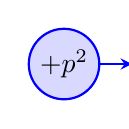
\begin{tikzpicture}[baseline=(R.base)]
                \node[draw=blue, fill=blue!15, circle, inner sep=2pt, thick] (R) {$+ p^2$};
                % L'overlay evita che la freccia sposti il cerchio a sinistra
                \draw[blue, thick, ->, >=stealth, overlay] (R.east) -- ++(0.4,0) node[right] {R(p)};
            \end{tikzpicture}
        & & 
\end{array}
$
\end{center}

\item \textbf{Si somma}: $\textcolor{red}{M(p)} +p^k\textcolor{blue}{R(p)}$
       $$X_M(p)=\textcolor{red}{M(p)}+p^4\textcolor{blue}{R(p)} = \textcolor{red}{1+p+p^3} + \textcolor{blue}{p^6}$$
       $$X=\textcolor{red}{1101}\textcolor{blue}{001}$$
   \end{enumerate}

\end{esempio}

\subsection{Codici Ciclici - Algoritmi di decodifica e rilevazione di errore}
Ad ogni messaggio inviato $X$, associamo il polinomio $Y(p)$ associato al vettore ricevuto al canale. Per individuare un eventuale errore sarà necessario calcolare il polinomio \textbf{sindrome $s(p)$} di grado minore di $(n-k)$ associato a $Y(p)$. La sindrome si ottiene come \textbf{resto} della divisione polinomiale tra $Y(p)$ e $G(p)$.

$$Y(p)= Q(p)G(p)+s(p)$$
Solamente in caso di \textbf{sindrome nulla}, la parola di codice è valida, in quanto il polinomio generatore $G(p)$ è un \textbf{fattore} di $Y(p)$.

Ciò è conseguenza del seguente teorema:

\textbf{Teorema:} Sia $C$ un codice ciclico $(n,k)$, con polinomio di controllo di parità $H(p)$. Un polinomio $Y(p)$ è un polinomio di codice se e soltanto se:
\[Y(p)H(p) \equiv 0 \pmod{p^n-1}\]
Per un codice $(n,k)$ e capacità correttiva pari a $t$, il vettore di errore $E(p)$ sarà tale che:
$$X(p)= Y(p)+E(p)$$
\textbf{Teorema:} Se la sindrome $S(p)$, calcolata rispetto al polinomio $Y(p)$, ha \textbf{peso} $\leq t$, allora il vettore di errore coincide con la sindrome $E(p) = S(p)$.

Questa conseguenza è applicabile per la correzione \textbf{solamente se gli errori sono presenti nei primi $q$ bit del messaggio}. Si può però \textit{shiftare ciclicamente} $Y(p)$ fino ad ottenere, dopo $m$ shift, una sindrome $S_m(p)$ di peso minore o uguale a $t$.
Il \textit{nuovo} vettore di errore $E(p)$ sarà quindi pari alla sindrome shiftata di $m$ posizioni verso destra:
$$E(p)=p^mS_m(p)\mod(p^n-1)$$

\begin{esempio}{Algoritmo di decodifica}
    Codice di Hamming ciclico $(7,4)$, polinomio generatore $G(p)= 1 + p^2 +p^3$.
    \begin{itemize}
        \item $t=1$, si riceve la sequenza $Y=110\textcolor{red}{0}001$, polinomio associato $Y(p)= 1+p+p^6$.
        \item Polinomio sindrome $S(p)=p^2+1$ con peso $2>t$.
        \item Si opera uno shift a sinistra di una posizione $m=1$
        $$Y'= 10\textcolor{red}{0}0011 \implies Y'(p)= 1+p^5+p^6$$
        \item Il \textit{nuovo} polinomio sindrome è $S_1(p)=p^2$ ha peso $1=t$, e dunque:
        $$E(p)= p^mS_1(p)=p^3$$
        $$X(p)=Y(p)+E(p)= 1 + p +p^3+p^6$$
    \end{itemize}
\end{esempio}

\subsubsection{Codici BCH}
I codici \textbf{BCH} (Bose – Chaudhuri – Hocquenghem) sono codici ciclici, \textit{non necessariamente binari}, che costituiscono una generalizzazione dei codici di Hamming con $t \geq 1$.
Per $m \geq 3$ \textit{intero}, esiste un codice BCH binario con parametri:
\[ n=2^m-1, \quad n-k \leq mt, \quad d_{min} \geq 2t+1 \]
Può correggere $t$ errori.
Il corrispondente polinomio generatore si può costruire dai fattori di:
\[ p^n + 1 = p^{2^m-1} + 1 \]

\subsubsection{Esempi di polinomi generatori}
\definecolor{headergreen}{HTML}{1C714C}

\begin{center}
\renewcommand{\arraystretch}{1.5} % Aumenta l'altezza delle celle
\begin{tabular}{|c|c|c|c|c|r|}
    \hline
    % Riga di intestazione colorata
    \rowcolor{headergreen} 
    \textcolor{white}{\textbf{Codice}} & 
    \textcolor{white}{\textbf{$n$}} & 
    \textcolor{white}{\textbf{$k$}} & 
    \textcolor{white}{\textbf{$R_c$}} & 
    \textcolor{white}{\textbf{$d_{min}$}} & 
    \textcolor{white}{\textbf{$G(p)$}} \\ \hline
    
    % Blocchi Hamming
    \multirow{3}{*}{Hamming} & 7  & 4  & 0.57 & 3 & 1 011 \\ \cline{2-6}
                             & 15 & 11 & 0.73 & 3 & 10 011 \\ \cline{2-6}
                             & 31 & 26 & 0.84 & 3 & 100 101 \\ \hline
                             
    % Blocchi BCH
    \multirow{3}{*}{BCH}     & 15 & 7  & 0.46 & 5 & 111 010 001 \\ \cline{2-6}
                             & 31 & 21 & 0.68 & 5 & 11 101 101 001 \\ \cline{2-6}
                             & 63 & 45 & 0.71 & 7 & 1 111 000 001 011 001 111 \\ \hline
                             
    % Golay
    Golay                    & 23 & 12 & 0.52 & 7 & 101 011 100 011 \\ \hline
\end{tabular}
\end{center}

\subsubsection{Esempio di codice ciclico binario}
Si considera un codice ciclico binario di lunghezza $7$.
$$x^7 -1 =(x-1)(x^3 + x +1)(x^3 + x^2 + 1)$$
\textit{Lavorando con codici binari, i segni "$+$" e "$-$" sono intercambiabili}:
$$x^7 +1 =(x+1)(x^3 + x +1)(x^3 + x^2 + 1)$$
Abbiamo quindi tre fattori irriducibili e, di conseguenza, $2^3=8$ codici ciclici (inclusi $g(x)=1$ e $g(x)= x^7+1$):
\begin{center}
\renewcommand{\arraystretch}{1.2}
\[
\begin{aligned}
    (i)   \quad & 1 = 1 \\
    (ii)  \quad & x + 1 = x + 1 \\
    (iii) \quad & x^3 + x + 1 = x^3 + x + 1 \\
    (iv)  \quad & x^3 + x^2 + 1 = x^3 + x^2 + 1 \\
    (v)   \quad & (x + 1)(x^3 + x + 1) = x^4 + x^3 + x^2 + 1 \\
    (vi)  \quad & (x + 1)(x^3 + x^2 + 1) = x^4 + x^2 + x + 1 \\
    (vii) \quad & (x^3 + x + 1)(x^3 + x^2 + 1) = \\
                & \quad x^6 + x^5 + x^4 + x^3 + x^2 + x + 1 \\
    (viii)\quad & (x + 1)(x^3 + x + 1)(x^3 + x^2 + 1) = x^7 + 1
\end{aligned}
\]
\end{center}
\begin{itemize}
    \item $(i) \quad g(x) =1$ genera tutte le parole di lunghezza 7.
    \item $(ii) \quad g(x) =1+x$ genera un codice di controllo con una cifra di parità.
    \item $(vii) \quad g(x) = 1+x + x^2+x^3+x^4+x^5+x^6$ genera un codice a ripetizione con $k=1$ (un solo bit di informazione ripetuto 7 volte)
    \item $(viii) \quad g(x) =1+x^7$ si ha il codice $0$
    \item $(iii) \quad g(x) = x^3+x+1$ ha grado $3$, può generare codici di Hamming($7,4$).
    \item $(iv) \quad g(x) = x^3+x^2+1$ ha grado $3$, può generare codici di Hamming($7,4$).
    \item $(v) \quad g(x) = (x+1)(x^3+x+1)=x^4+x^3+x^2+1$ genera il codice duale di Hamming.
    \item $(vi) \quad g(x) = (x+1)(x^3+x^2+1)=x^4+x^2+x+1$ genera il codice duale di Hamming.
\end{itemize}

\subsection{Vantaggi dei codici ciclici}
Sono tre i vantaggi garantiti dall'impiego di codici ciclici:
\begin{enumerate}
    \item semplicità di codifica;
    \item semplicità nel calcolo della sindrome;
    \item una struttura matematica precisa che consente di sviluppare metodi di decodifica molto efficienti, in quanto non è più necessario \textit{memorizzare informazione}; è quindi possibile implementare codici con
    $$n>>1,k>>1 \implies R_c \approxeq 1$$
\end{enumerate}
\subsubsection{Osservazioni}
\begin{itemize}
    \item Se il polinomio $G(p)$ divide sia $(p^m+1)$ che  $(p^n+1)$, con $m<n$, allora $(p^m+1)$ è una codeword generata dal polinomio generatore.
    \item $p^m+1$ è il polinomio della codeword di peso $2$ per il codice $(n,k)$, il quale ha quindi di conseguenza distanza minima $d_{min}\leq2$
    \item Conseguentemente tale codice potrà rilevare \textbf{al massimo} un singolo errore
    \item Per aggirare questa limitazione il parametro $n$ deve essere il più piccolo intero tale che $(p^n +1)$ è \textbf{multiplo} di $G(p)$.
\end{itemize}